{
  \par\vspace{5mm}
  {\large \textbf{Table Sorting and Filtering}}
  \par\vspace{3mm}

  In this section, users can sort and filter the data to view the results based on specific criteria.
  \par\vspace{3mm}
  \textbf{1. Sorting:}
  Users can click on the **column headers** to sort the data in ascending or descending order. This allows for a better-organized view of the data according to the selected column.
  \par\vspace{2mm}
  \textbf{2. Filtering}:
  Users can apply custom filters to the displayed results by using the filter icon. By clicking on the **filter icon** (highlighted in the image), a dropdown menu appears where users can search for specific values and select which options they want to filter by. This feature allows users to focus on the data they are interested in, such as selecting specific operators (e.g., **Banglalink**, **Grameenphone**, **Teletalk**).

  \begin{figure}[H]
    \centering
    \colorbox{gray!20}{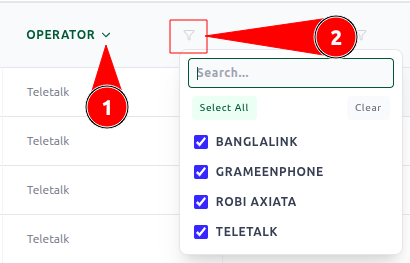
\includegraphics[width=.25\textwidth]{img/common/commonarea/results/R4TableSortingFilter.png}}  % Replace with the path to your image file
    \caption{Example of Table Sorting and Filtering}
  \end{figure}
}